\chapter{Popis polohy a směru v prostoru}

\section{Vektory}

Polohu a směr v~prostoru určujeme pomocí vektorů. Vektory značíme tučně $\vect{v}$ (případně se šipkou $\vec{v}$), jejich velikost jako $|\vect{v}|$ (nebo prostým písmem $v$) a směr pomocí jednotkového vektoru $\vect{v}/|\vect{v}|$.

\subsection{Vektorová aritmetika a kartézská soustava souřadnic}

Vektory můžeme vyjádřit v~tzv.~\emph{kartézské soustavě souřadnic}:
$$ \vect{v} = v_x\vect{e}_x + v_y\vect{e}_y + v_z\vect{e}_z, $$
nebo zkráceně pomocí uspořádané trojice složek $\vect{v} = (v_x, v_y, v_z)$, kde $\vect{e}_x, \vect{e}_y, \vect{e}_z$ (často značené též $\vect{i}, \vect{j}, \vect{k}$) jsou \emph{ortonormální bázové vektory} -- vzájemně kolmé jednotkové vektory ve směrech jednotlivých souřadnicových os.

Základní operace s~vektory:
\begin{description}
    \item[Velikost vektoru (eukleidovská norma):]
    $$ |\vect{a}| = \sqrt{a_x^2 + a_y^2 + a_z^2} $$
    \item[Součet vektorů a násobení skalárem:]
    $$ \vect{a} + \vect{b} = (a_x + b_x,\, a_y + b_y,\, a_z + b_z) $$
    $$ c \vect{a} = (c a_x,\, c a_y,\, c a_z) $$
    \item[Skalární součin:]
    $$ \vect{a}\cdot\vect{b} = a_x b_x + a_y b_y + a_z b_z = \sum_{i=1}^{3} a_i b_i = a_i b_i, $$
    kde v~posledním výrazu je využita Einsteinova sumační konvence. Geometricky platí
    $$ \vect{a}\cdot\vect{b} = |\vect{a}|\,|\vect{b}|\cos\phi, $$
    kde $\phi \in [0, \pi]$ je úhel sevřený vektory $\vect{a}$ a $\vect{b}$.
    \item[Vektorový součin:]
    $$ \vect{a} \times \vect{b} = \begin{vmatrix}
        \vect{i} & \vect{j} & \vect{k} \\
        a_x & a_y & a_z \\
        b_x & b_y & b_z
    \end{vmatrix} = (a_y b_z - a_z b_y,\, a_z b_x - a_x b_z,\, a_x b_y - a_y b_x). $$
\end{description}

\begin{center}
    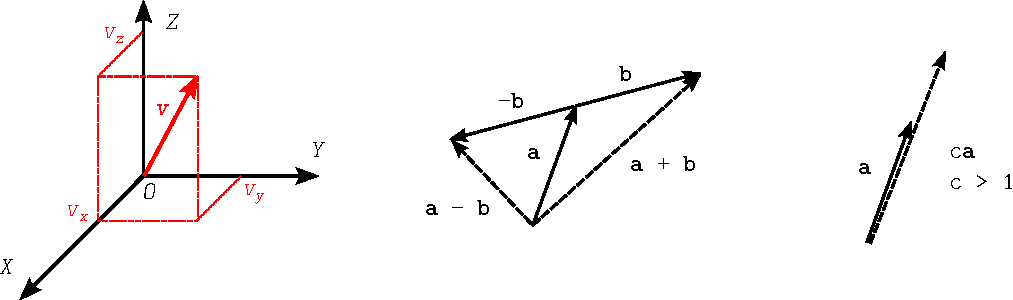
\includegraphics[width=0.9\textwidth]{chapters/figures/vektory.pdf}
\end{center}

Skalárním součinem vektoru s~jednotkovými bázovými vektory $\vect{i}, \vect{j}, \vect{k}$ získáme tzv.~\emph{směrové kosiny} (při označení velikosti $|\vect{a}| = a$):
$$ \vect{a}\cdot\vect{i} = a\cos\alpha,\quad \vect{a}\cdot\vect{j} = a\cos\beta,\quad \vect{a}\cdot\vect{k} = a\cos\gamma, $$
pro které z~vlastností eukleidovské normy plyne identita
$$ \cos^2\alpha + \cos^2\beta + \cos^2\gamma = 1. $$

Geometrická interpretace vektorového součinu:

\begin{center}
    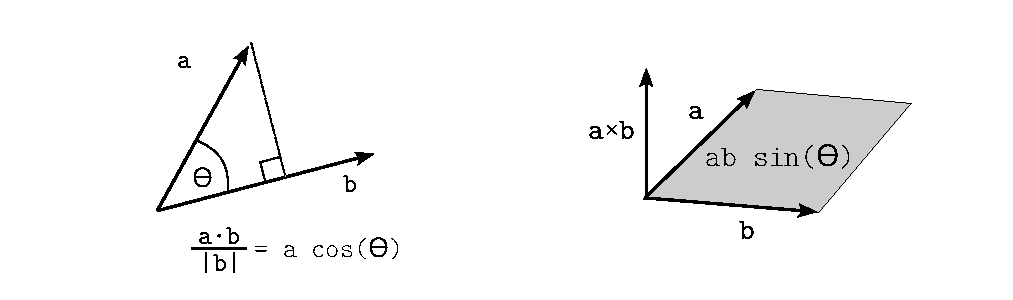
\includegraphics[width=0.9\textwidth]{chapters/figures/vektory_soucin.pdf}
\end{center}

Vektorový součin vytváří v~prostoru orientovanou trojici vektorů, která určuje tzv.~\emph{pravotočivou soustavu souřadnic} (na obrázku vpravo). Orientaci výsledného vektoru určuje \emph{pravidlo pravé ruky}: natáhneme-li palec, ukazovák a prostředník pravé ruky do vzájemně kolmých směrů tak, aby ukazovák mířil ve směru prvního vektoru $\vect{a}$ a prostředník ve směru druhého vektoru $\vect{b}$, pak vztyčený palec ukazuje směr vektorového součinu $\vect{a}\times\vect{b}$ (ekvivalentně: sevřeme-li prsty pravé ruky ve směru od $\vect{a}$ k~$\vect{b}$ přes menší z~úhlů, palec míří ve směru $\vect{a}\times\vect{b}$).

\begin{center}
    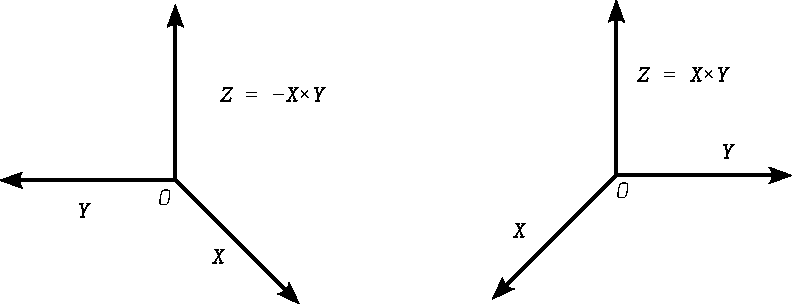
\includegraphics{chapters/figures/vektory_RL.pdf}
\end{center}

Ve fyzice se standardně používají pravotočivé soustavy. Levotočivé soustavy se naproti tomu uplatňují například v~některých konvencích počítačové grafiky.

\subsection{Kroneckerův a Levi-Civitův symbol}
V~kombinaci s~Einsteinovou sumační konvencí (automatické sčítání přes opakující se indexy přes rozsah $1, 2, 3$) lze řadu vektorových operací se složkami zapsat velmi kompaktně pomocí \emph{Kroneckerova symbolu} $\delta_{ij}$ a \emph{Levi-Civitova symbolu} $\varepsilon_{ijk}$.

Pro Kroneckerův symbol platí:
$$ \delta_{ij} = \begin{cases} 1 & \text{pro } i=j, \\ 0 & \text{pro } i \neq j. \end{cases} $$

Levi-Civitův symbol $\varepsilon_{ijk}$ je \emph{totálně antisymetrický tenzor 3.~řádu}:
\begin{itemize}
    \item $\varepsilon_{ijk} = 0$, pokud se alespoň dva z~indexů $i, j, k$ rovnají (např.~$\varepsilon_{112} = \varepsilon_{313} = 0$),
    \item $\varepsilon_{123} = 1$ a pro všechny ostatní sudé permutace indexů platí $\varepsilon_{123} = \varepsilon_{231} = \varepsilon_{312} = 1$,
    \item pro liché permutace indexů platí $\varepsilon_{213} = \varepsilon_{132} = \varepsilon_{321} = -1$.
\end{itemize}

Skalární součin lze zapsat pomocí Kroneckerova symbolu jako $\vect{a}\cdot\vect{b} = \delta_{ij} a_i b_j = a_i b_i$. Složka vektorového součinu $\vect{c} = \vect{a}\times\vect{b}$ se vyjádří jako
$$ c_i = \varepsilon_{ijk} a_j b_k. $$

Mezi součiny Levi-Civitových symbolů platí mimořádně užitečná kontrakční identita:
$$ \varepsilon_{ijk}\varepsilon_{ilm} = \delta_{jl}\delta_{km} - \delta_{jm}\delta_{kl}. $$

\begin{priklad}[Dvojný vektorový součin a identita BAC-CAB]
    Vyjádřete složky dvojného vektorového součinu $\vect{a} \times (\vect{b}\times\vect{c})$ pomocí indexového zápisu.

    \textbf{Řešení:} Označme $\vect{d} = \vect{b} \times \vect{c}$, pak $d_m = \varepsilon_{mjk} b_j c_k$. Pro $i$-tou složku vektoru $\vect{v} = \vect{a} \times \vect{d}$ dostáváme:
    $$ v_i = \varepsilon_{ilm} a_l d_m = \varepsilon_{ilm} \varepsilon_{mjk} a_l b_j c_k = \varepsilon_{mil} \varepsilon_{mjk} a_l b_j c_k. $$
    Protože cyklická záměna indexů nemění hodnotu ($\varepsilon_{ilm} = \varepsilon_{mil}$), uplatníme kontrakční identitu pro společný index $m$:
    $$ \varepsilon_{mil}\varepsilon_{mjk} = \delta_{ij}\delta_{lk} - \delta_{ik}\delta_{lj}. $$
    Dosazením získáme:
    \begin{align*}
        v_i &= (\delta_{ij}\delta_{lk} - \delta_{ik}\delta_{lj}) a_l b_j c_k \\
            &= \delta_{ij} b_j \, \delta_{lk} a_l c_k - \delta_{ik} c_k \, \delta_{lj} a_l b_j \\
            &= b_i (a_k c_k) - c_i (a_j b_j) \\
            &= b_i (\vect{a}\cdot\vect{c}) - c_i (\vect{a}\cdot\vect{b}).
    \end{align*}
    Ve vektorovém zápisu jsme tak dokázali známou identitu:
    $$ \vect{a}\times(\vect{b}\times\vect{c}) = \vect{b}(\vect{a}\cdot\vect{c}) - \vect{c}(\vect{a}\cdot\vect{b}). $$
\end{priklad}

\section{Křivočaré soustavy souřadnic: cylindrické a sférické}

Pro konkrétní vyjádření polohových a jiných vektorů volíme souřadnicovou soustavu. Na základě symetrie problému nebo kvůli snazšímu řešení pohybových rovnic volíme vedle kartézských souřadnic libovolné obecné (křivočaré) souřadnice $q_1, q_2, q_3$, které lze vzájemně jednoznačně převádět do kartézských souřadnic a zpět:
$$ q_1 = q_1(x, y, z),\quad q_2 = q_2(x, y, z),\quad q_3 = q_3(x, y, z) $$
a
$$ x = x(q_1, q_2, q_3),\quad y = y(q_1, q_2, q_3),\quad z = z(q_1, q_2, q_3). $$

Nejčastěji používanými křivočarými soustavami jsou souřadnice cylindrické (ve 2D polární) a sférické.

\subsection{Cylindrické (polární) souřadnice}
Cylindrické souřadnice bodu v~prostoru jsou definovány pomocí poloměru (vzdálenosti od osy $z$) $\rho \ge 0$, azimutálního úhlu $\phi \in [0, 2\pi)$ a výšky $z \in \mathbb{R}$. Převodní vztahy do kartézských souřadnic jsou:
$$ x = \rho\cos\phi,\quad y = \rho\sin\phi,\quad z = z, $$
a zpětný převod má tvar:
$$ \rho = \sqrt{x^2 + y^2},\quad \phi = \operatorname{atan2}(y, x),\quad z = z, $$
kde funkce $\operatorname{atan2}(y, x)$ představuje rozšířený arkustangens se správným určením kvadrantu (na rozdíl od prostého $\arctan(y/x)$, který dává hodnoty pouze v~rozsahu $(-\pi/2, \pi/2)$ a pro $x < 0$ je k~němu nutné přičíst $\pi$).

\begin{center}
    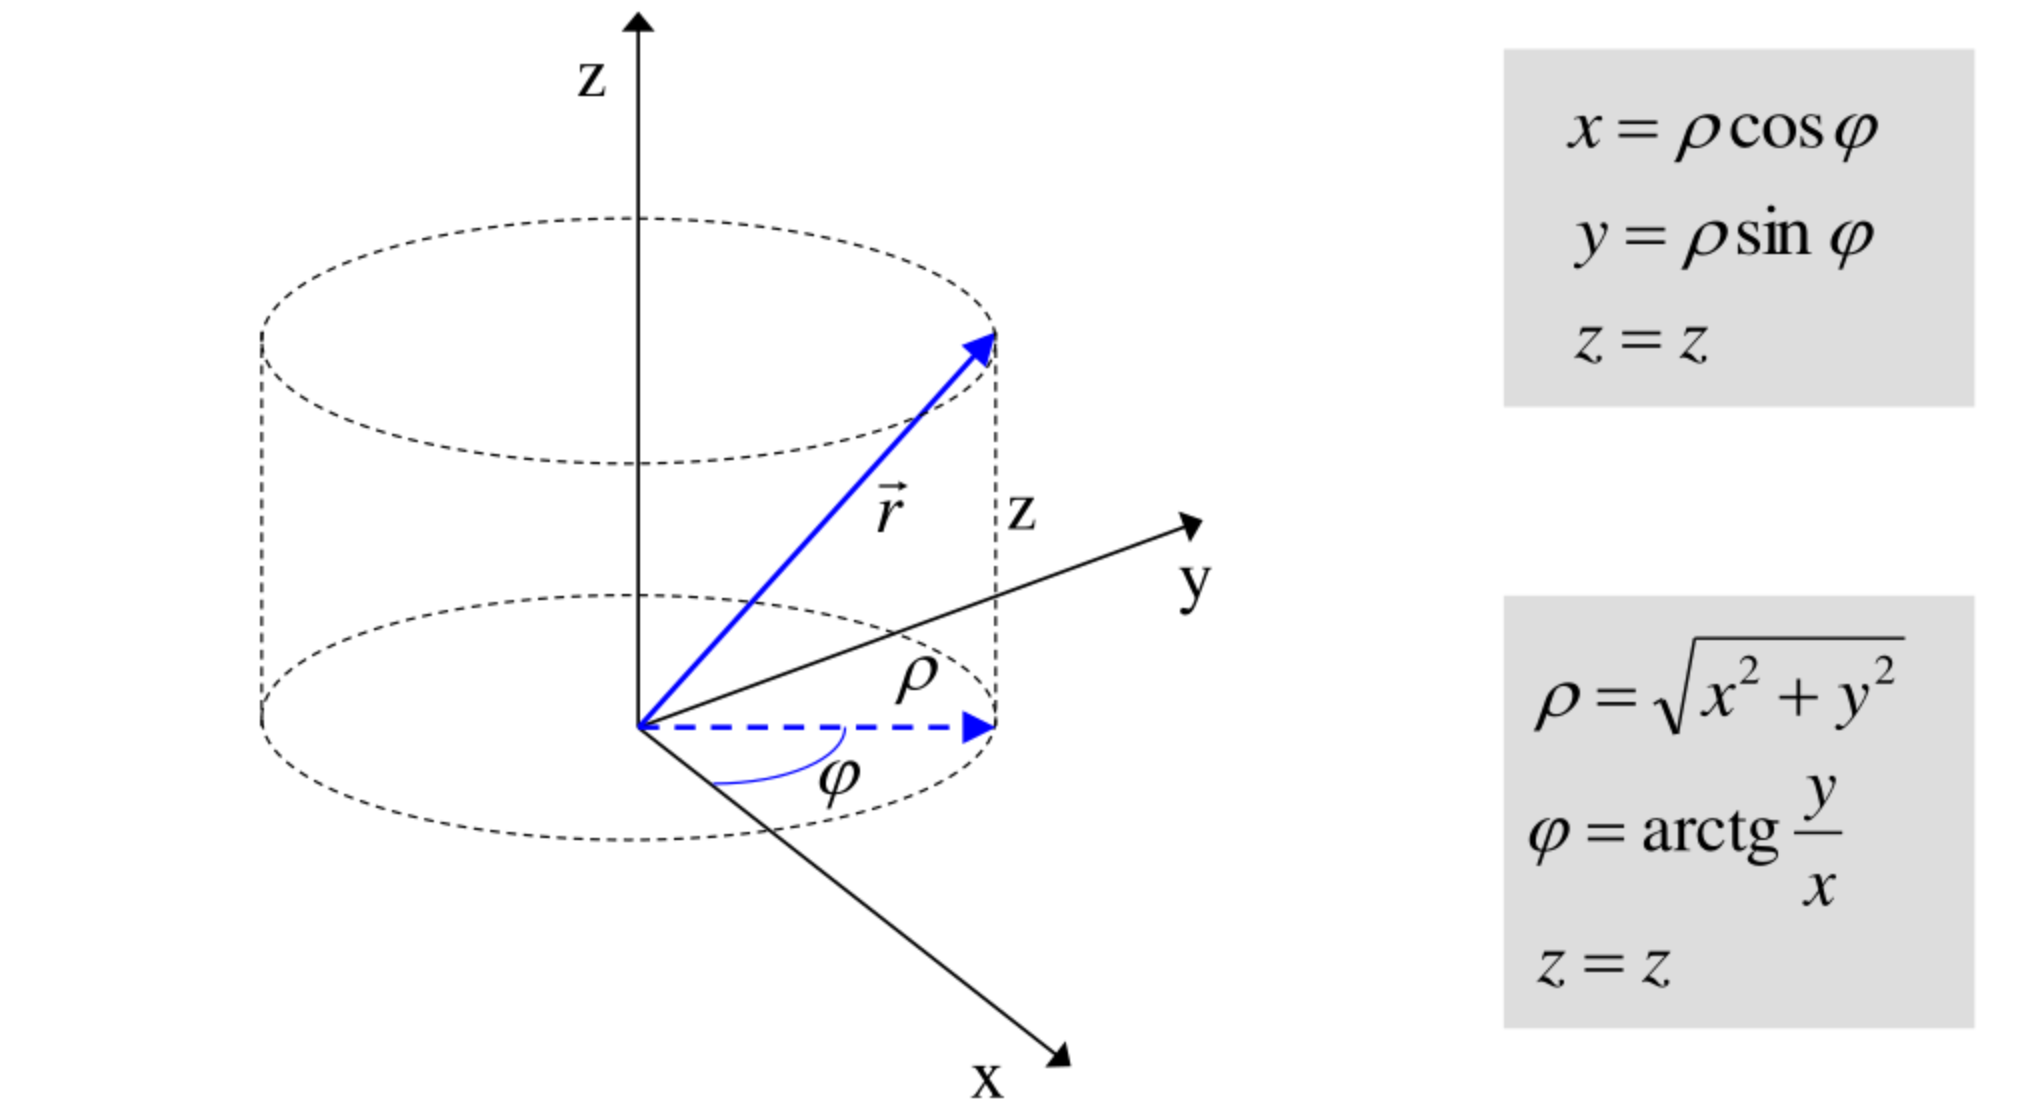
\includegraphics[width=0.9\textwidth]{chapters/figures/cylindr.png}
\end{center}

\subsection{Sférické souřadnice}

Sférické souřadnice jsou určeny radiální vzdáleností $r \ge 0$ (vzdálenost od počátku), polárním (zenitovým) úhlem $\theta \in [0, \pi]$ (úhel odklonu od kladné poloosy $z$) a azimutálním úhlem $\phi \in [0, 2\pi)$ v~rovině $xy$ měřeným od osy $x$ (analogie zeměpisné délky):
\begin{align*}
    x &= r \sin\theta \cos\phi,\\
    y &= r \sin\theta \sin\phi,\\
    z &= r \cos\theta,
\end{align*}
a pro inverzní transformaci platí:
\begin{align*}
    r &= \sqrt{x^2 + y^2 + z^2}, \\
    \phi &= \operatorname{atan2}(y, x), \\
    \theta &= \arccos\left(\frac{z}{r}\right).
\end{align*}

Polární úhel $\theta$ se ve fyzice a matematice standardně měří od svislé osy $z$ (od „severního pólu“, $\theta \in [0, \pi]$). V~geografii se naproti tomu zeměpisná šířka $\vartheta$ měří od rovníku (v~intervalu $[-\pi/2, \pi/2]$); v~takovém případě by bylo $z = r\sin\vartheta$.

\begin{center}
    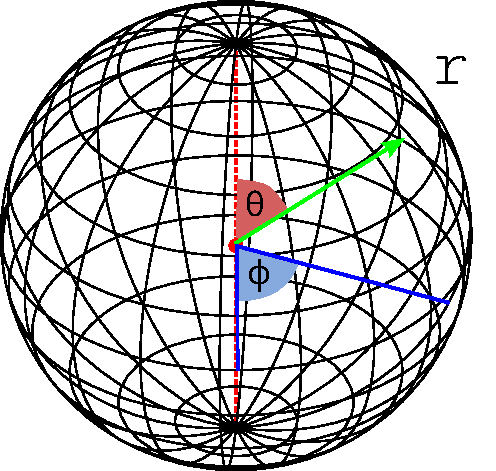
\includegraphics{chapters/figures/sfericke.pdf}
\end{center}

\section{Transformace souřadnic}

Uvažujme soustavu bodů popsanou polohovými vektory $\vect{r}_k$. Tuto soustavu můžeme popsat v~různě zvolených souřadnicových soustavách, které vznikly z~původní soustavy určitou transformací:
\begin{itemize}
    \item \emph{posunutí (translace) soustavy o~vektor $\vect{p}$:} souřadnice bodu se transformují podle $\vect{r}' = \vect{r} - \vect{p}$,
    \item \emph{škálování souřadnic konstantou $c$:} $\vect{r}' = c\vect{r}$ (případně $\vect{r}' = \frac{1}{c}\vect{r}$ při změně jednotek délky),
    \item \emph{otočení (rotace) a zrcadlení soustavy}.
\end{itemize}

Uvažujme otočení souřadnicové soustavy kolem osy $z$ o~úhel $\alpha$ proti směru hodinových ručiček. Původní souřadnice bodu označme $\vect{r} = (x, y, z)$. V~nové pootočené soustavě bude mít tentýž bod souřadnice $\vect{r}' = (x', y', z')$, pro něž platí:
\begin{align*}
    x' &= x \cos\alpha + y\sin\alpha,\\
    y' &= -x \sin\alpha + y\cos\alpha,\\
    z' &= z.
\end{align*}

\begin{center}
    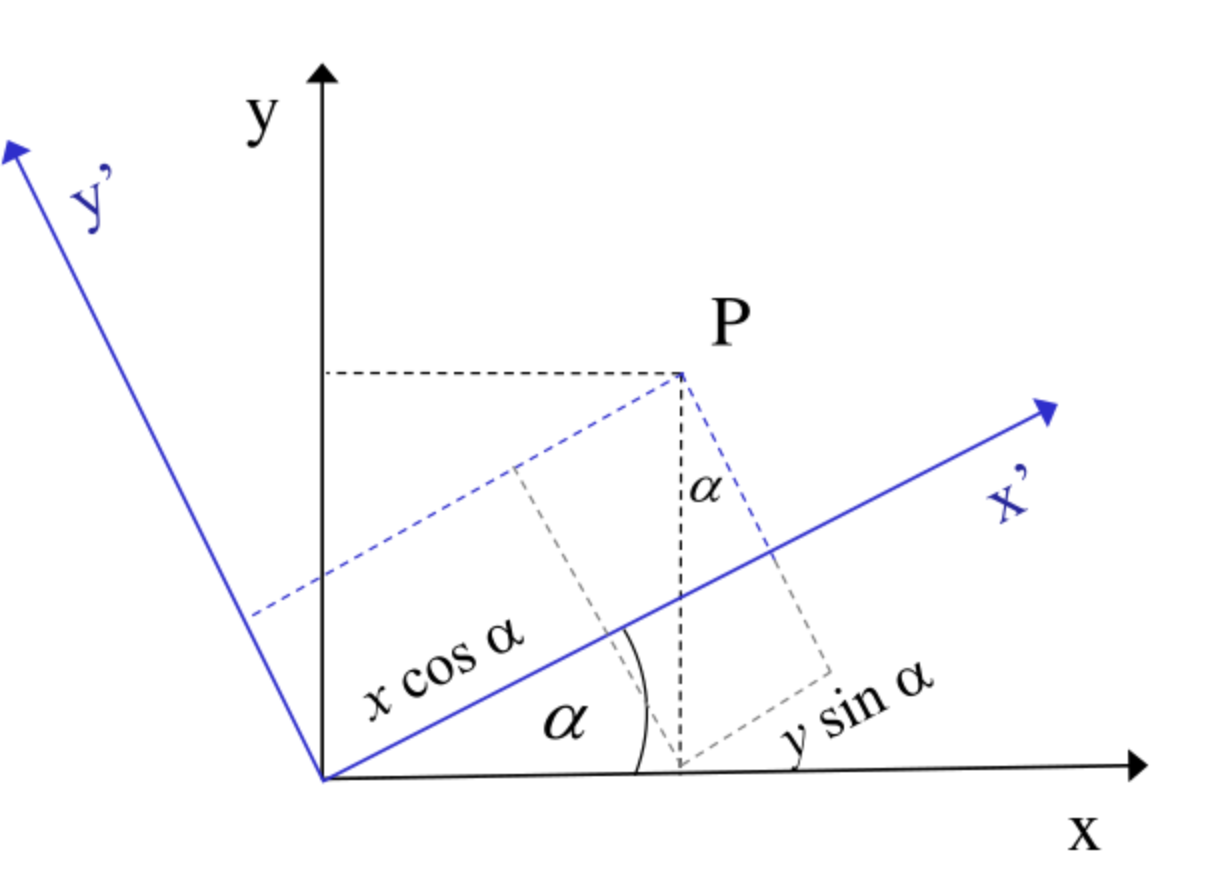
\includegraphics[width=0.75\textwidth]{chapters/figures/rotace_soustavy.png}
\end{center}

Tento vztah lze zapsat také maticově:
$$ 
    \begin{pmatrix}
        x' \\ y' \\ z'
    \end{pmatrix} =  
    \begin{pmatrix}
        \cos\alpha & \sin\alpha & 0\\
        -\sin\alpha & \cos\alpha & 0 \\
        0 & 0 & 1
    \end{pmatrix}
    \begin{pmatrix}
        x \\ y \\ z
    \end{pmatrix},
$$
neboli v~indexovém zápisu
$$ r'_i = M_{ij} r_j. $$

Matice rotace je ortogonální ($M^{-1} = M^\mathsf{T}$, $\det M = 1$).
Také stejnolehlost (izotropní škálování) lze zapsat maticově pomocí jednoduché diagonální matice:
$$ M = \begin{pmatrix}
    c & 0 & 0\\
    0 & c & 0\\
    0 & 0 & c
\end{pmatrix}, $$
a zrcadlení např.~vůči rovině $xy$ má matici
$$ M=\begin{pmatrix}
    1 & 0 & 0\\
    0 & 1 & 0\\
    0 & 0 & -1
\end{pmatrix}, $$
přičemž pro zrcadlení platí $\det M = -1$ (mění orientaci prostoru z~pravotočivé na levotočivou).

Obecně lze všechny kombinace rotací, škálování a zrcadlení vyjádřit jednoduše pomocí násobení matic (lineární transformace). Spolu s~translací pak tvoří obecné afinní transformace eukleidovského prostoru.